\documentclass[a4paper,11pt]{scrartcl}

\usepackage[utf8]{inputenc}
\usepackage[ngerman]{babel}
\usepackage[T1]{fontenc}
\usepackage{amsmath}
\usepackage{graphicx}
\usepackage{tabularx}
\usepackage[a4paper, left=2cm, right=2cm, top=2.8cm, bottom=2.8cm]{geometry}
\usepackage{tikz}   
\usepackage[scaled]{helvet}
\usepackage{tabto} 
\usepackage{fancyhdr}
\usepackage{multirow}

\renewcommand*{\familydefault}{\sfdefault}

\pagestyle{fancy}

\setkomafont{section}{\huge}
\setkomafont{subsection}{\Large}


\lhead{Maximilian Hoffmann}
\chead{Betrieblicher Auftrag \\ \textbf{Kabeltester}}
\rhead{
\includegraphics[width=3cm]{Bilder/BMK_LOGO.png}}

%%%%%%%%%%%%%%%%%%%%%%%%%%%%%%%%%%%%%%%%%%%%%%%%%%%%%%%%%%%%%%%%%%%%%%%%%%%%%%%%%%%%%%%%%%%%%%%%%%%%%%%%%%%%%%%%%%%%%%%%%%%%%%%%%%%%%%%%%%%%%%%																																			 %
%														Funktionen der Schaltung															%
%																																		     %
%%%%%%%%%%%%%%%%%%%%%%%%%%%%%%%%%%%%%%%%%%%%%%%%%%%%%%%%%%%%%%%%%%%%%%%%%%%%%%%%%%%%%%%%%%%%%%%%%%%%%%%%%%%%%%%%%%%%%%%%%%%%%%%%%%%%%%%%%%%%%%

\begin{document}

%%%%%%%%%%%%%%%%%%%%%%%%%%%%%%%%%%%%%%%%%%%%%%%%%%%%%%%%%%%%%%%%%%%%%%%%%%%%%%%%%%%%%%%%%%%%%%%%%%%%%%%%%%%%%%%%%%%%%%%%%																																						%
%														Versorgung														%
%																														%
%%%%%%%%%%%%%%%%%%%%%%%%%%%%%%%%%%%%%%%%%%%%%%%%%%%%%%%%%%%%%%%%%%%%%%%%%%%%%%%%%%%%%%%%%%%%%%%%%%%%%%%%%%%%%%%%%%%%%%%%%

\section{Schaltplanentwurf}

\subsection{Versorgung}

\subsubsection{Schutzbeschaltung}

\begin{center}
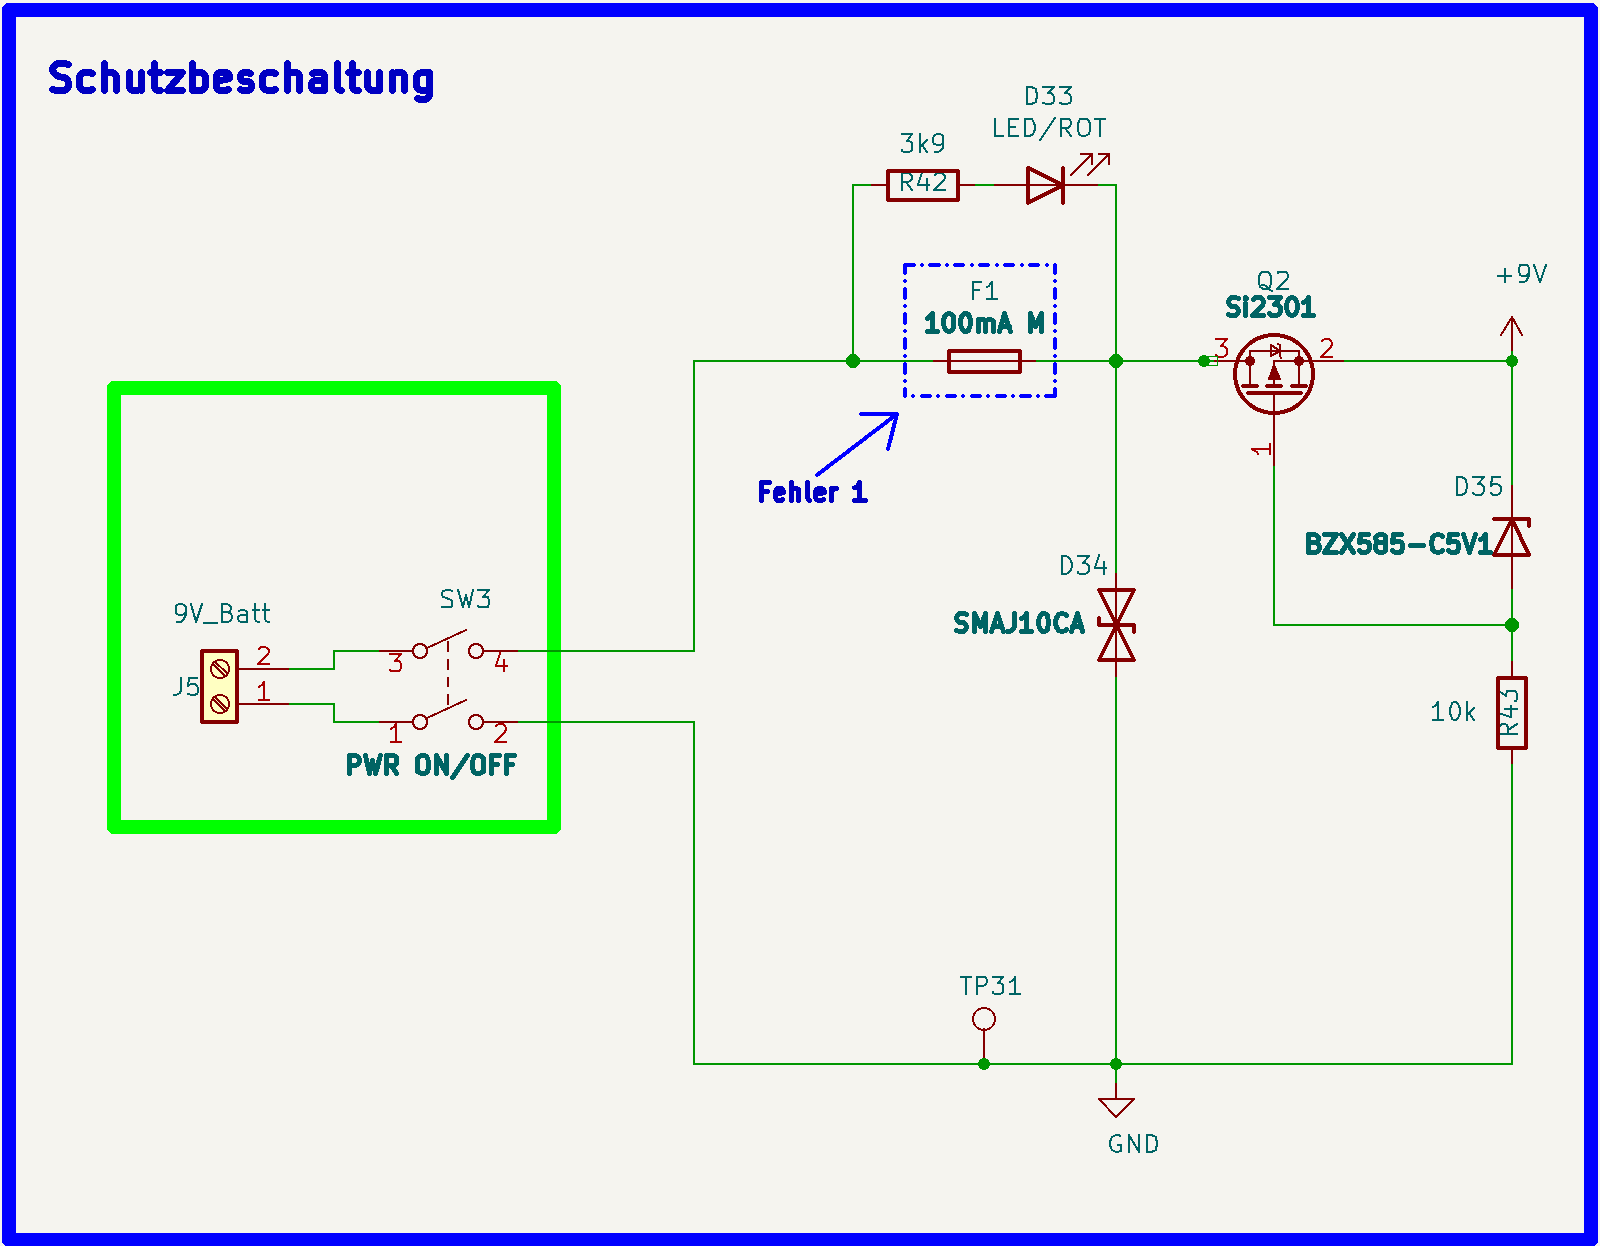
\includegraphics[width=10cm]{Bilder/Schutzbeschaltung.png}
\end{center}

Um die Schaltung zu schützen, wurde auf eine umfangreiche Eingangsschutzbeschaltung gesetzt. Die Versorgungsspannung kann dabei zweipolig durch den Schalter \glqq Power ON/OFF SW3 \grqq{} abgeschaltet werden.
\\
\\
Die mittelträge Sicherung F1, ist für den Überstromschutz verantwortlich. Löst diese aus, so fließt ein Strom über R42 und D33. Dabei wird der gesamte Stromfluss in der Schaltung auf ein Maximum von 2mA begrenzt. Als Ergebnis leuchtet D33 rot.
\\
Im Normalbetrieb werden R42 und D33 durch den ohmschen Widerstand der Sicherung F1 (12R) überbrückt.
\\
\\
Um den Eingang des DC/DC Wandlers vor Überspannungsspitzen zu schützen, kommt eine 10V TVS Diode zum Einsatz. Die Eingangsspannung dieser Schaltung wird dadurch auf ein Spannungsmaximum von 10V begrenzt. 
\\
\\
Da es bei einer Batterieanwendung sehr schnell zu einer ungewollten Verpolung der Anschlüsse kommen kann, wird ein Verpolungsschutz benötigt.
\\
Liegt eine korrekt gepolte Spannung an, so fließt der Strom durch die Z-Diode D35 und den strombegrenzenden Widerstand R43. Die über die Z-Diode abfallende Spannung von 5,1V, liegt somit auch an den Anschlüssen \glqq Source und Gate \grqq{} des P-Channel MOSFET Q2 an.
In diesem Fall, liegt eine um ca. 5V negativere Spannung an Gate gegenüber Source an. Die Drain-Source Strecke leitet und es kann Strom fließen.
\\ 
Wird die Versorgungsspannung verpolt, so fließt der Strom durch den Widerstand R43 und durch die Diode D35. Die Diode D35 befindet sich dabei in Durchlassrichtung und besitzt somit die Eigenschaften einer Si-Diode.
Die Spannung an dem Gate ist dabei um ca. 5V positiver gegenüber Source. Der P-Channel MOSFET sperrt und unterbindet einen Stromfluss.
\\

\subsubsection{DC/DC Wandler}

\begin{center}
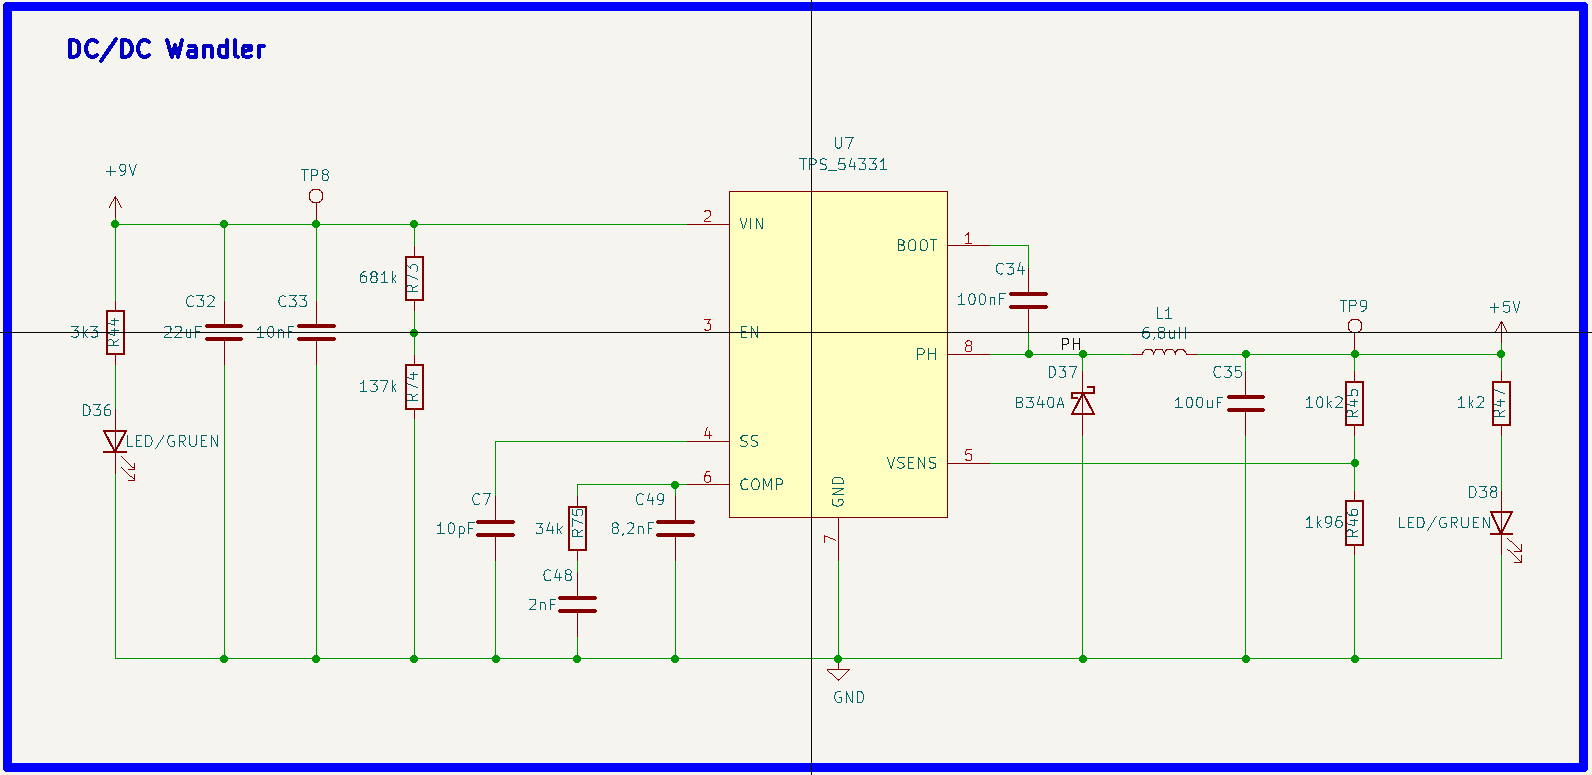
\includegraphics[width=16cm]{Bilder/DCDCWandler.png}
\end{center}

Bei der Auswahl des DC/DC Wandlers wurde auf die Verfügbarkeit bei BMK im Haus geachtet.
\\
Die Dimensionierung der externen Bauelemente wurde mit Hilfe des \glqq Texas Instruments Power Designer\grqq{} Web-Tool durchgeführt.
\\
Die grünen LED's D36 und D38 sorgen für ein optisches Feedback der Versorgungsspannungen.
\\
Allgemein wurde der Wandler für eine Ausgangsspannung von +5V und einen Ausgangsstrom von ca. 1,5A dimensioniert. Mit den Widerständen R73 und R74 kann der Schaltregler bei Über/-Unterspannung abschalten. Dafür wird eine oberer sowie untere Schaltschwelle berechnet.

\begin{center}
\begin{align}
	R73 &= \dfrac{V_{\Delta}}{3uA} = \dfrac{2V}{3uA} = 666k  \Rightarrow 680k\\
	R74 &= \dfrac{1,25V}{\dfrac{Vs - 1,25V}{R73} + 1uA} = \dfrac{1,25V}{\dfrac{8V - 1,25V}{680k} + 1uA} = 126k \Rightarrow 150k	\\
	V_{OUT}	&= V_{REF} + (\dfrac{R45}{R46} + 1) = 0,8V + (\dfrac{10,2k}{1,96k} + 1) = 4,96V
\end{align}
\end{center}


\newpage

%%%%%%%%%%%%%%%%%%%%%%%%%%%%%%%%%%%%%%%%%%%%%%%%%%%%%%%%%%%%%%%%%%%%%%%%%%%%%%%%%%%%%%%%%%%%%%%%%%%%%%%%%%%%%%%%%%%%%%%%%																																						%
%														NE555 Taktgeber													%
%																														%
%%%%%%%%%%%%%%%%%%%%%%%%%%%%%%%%%%%%%%%%%%%%%%%%%%%%%%%%%%%%%%%%%%%%%%%%%%%%%%%%%%%%%%%%%%%%%%%%%%%%%%%%%%%%%%%%%%%%%%%%%

\subsection{NE555 Taktgeber}

\subsubsection{Takt}

\begin{center}
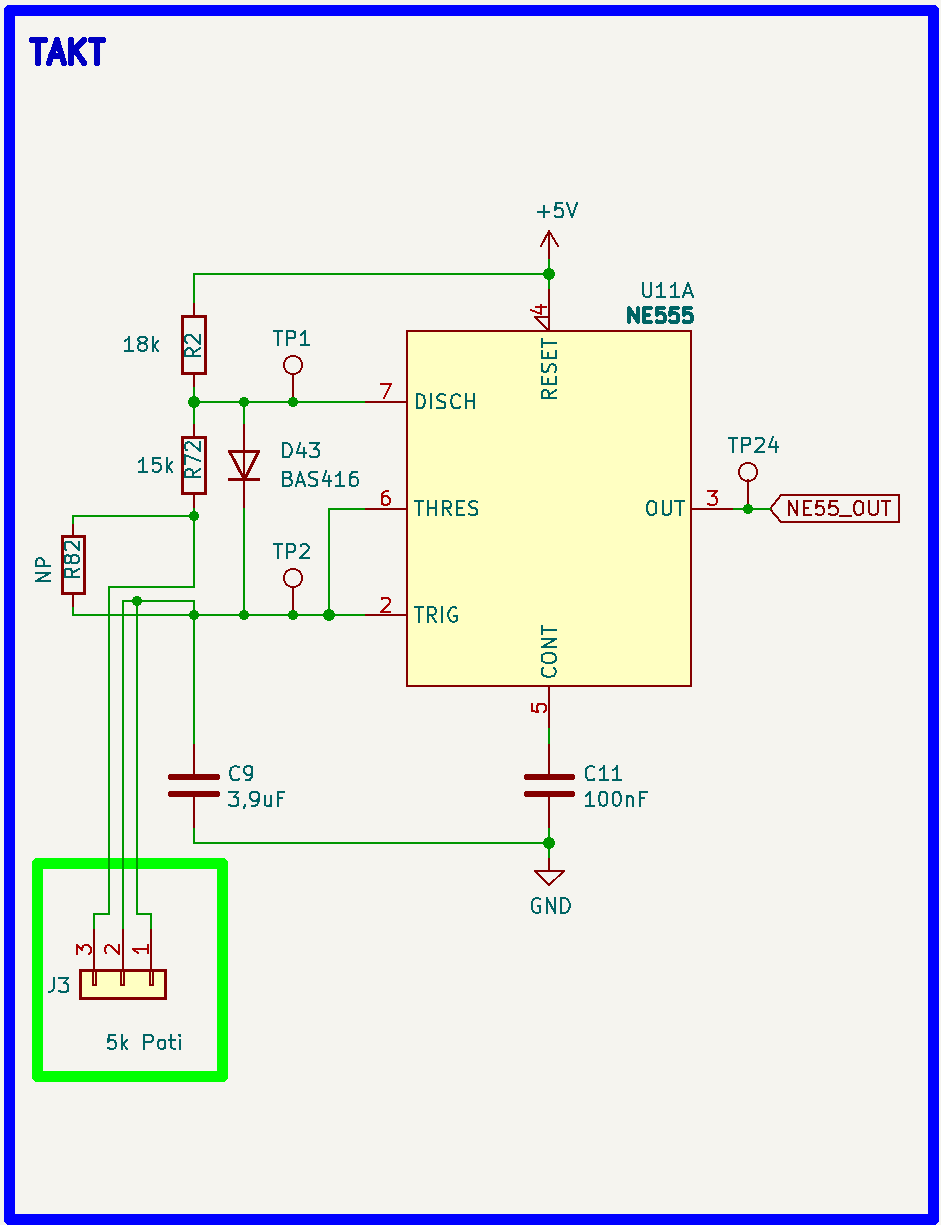
\includegraphics[width=10cm]{Bilder/Takt.png}
\end{center}

Als Taktgeber kommt der \glqq NE555 \grqq{} zum Einsatz. Dieser wird als astabile Kippstufe betrieben. Mit Hilfe der Diode D43 gleichen sich Impulszeit und Pausenzeit an. Über das Poti (Connector) J3 soll die Ausgangsfrequenz auf ca. 10Hz eingestellt werden können. 
\\
\\
Im Einschaltmoment ist C9 entladen. Somit liegt das Signal am Triggereingang (PIN 2) unterhalb von $\frac{1}{3} VCC$. Das interne FlipFlop wird gesetzt und der Ausgang (PIN 3) erfährt einen High-Pegel. Der Kondensator C9 lädt sich nun über R2 und D43 auf. Der Ladevorgang hält so lange an, bis das Spannungspotential an Pin 6 (Threshold) einen höheren Wert als $\frac{2}{3} VCC$ aufweist. Das interne FlipFlop's wird zurückgesetzt und der Ausgang erfährt einen Low-Pegel. Der Kondensator C9 entlädt sich nun über R72 und den (auf GND durchgeschaltenen) Pin 7 (Discharge). Hat sich der Kondensator nun wieder auf ein Spannungspotential unterhalb von $\frac{1}{3}$ entladen, so wird er Ausgang wieder gesetzt und der Entladevorgang über Pin 7 unterbunden. Dieser Vorgang wiederholt sich solange Energie von außen hinzugefügt wird. 

\begin{center}
\begin{align}
	f_{OUT} &= \dfrac{1}{0,69*R2*C9 + 0,69*(R72+R_{J3})* C9} = \dfrac{1}{0,69*18k*3,9uF*2} = 10,3Hz
\end{align} 
\end{center}

\newpage
\subsubsection{Taktumschaltung}

\begin{center}
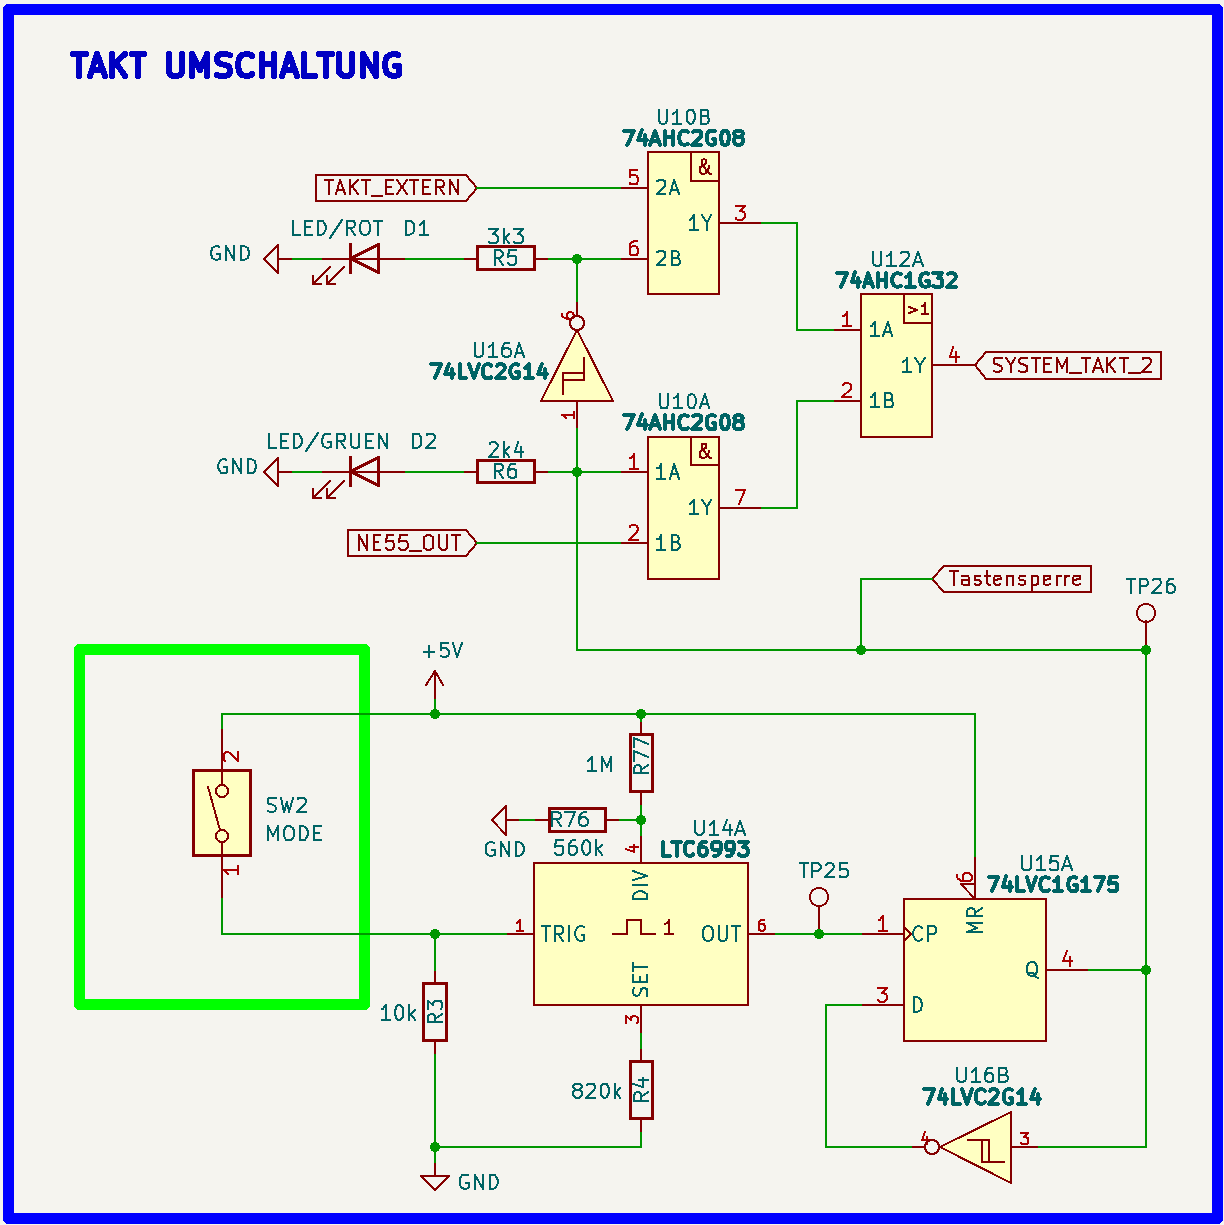
\includegraphics[width=13cm]{Bilder/Taktumschaltung.png}
\end{center}


\textbf{Funktionsbeschreibung LTC6993 U14}
\\
Das IC „LTC6993“ ist eine Monostabile Kippstufe mit einer einstellbaren Pulsweite von 1us – 33,6s. Dabei wird bei einem Impuls über den Trigger-Eingang (Pin 1), der Ausgangszustand für eine einstellbare Zeit gespeichert bevor der Ausgang wieder in den stabilen Zustand zurück kippt. Über die Außenbeschaltung der Pin’s „DIV“ und „SET“ kann die Pulsweite (Kipp-Zeit) konfiguriert werden. Der Pin „DIV“ ist dabei intern mit einem 4 Bit A/D-Wandler beschalten. Dieser führt drei seiner Datenleitungen einem Taktteiler zu. Dieser Taktteiler ist dadurch zwischen 1 und 2 097 152 einstellbar. Die vierte Datenleitung (MSB) übergibt ihren Zustand dem Block „Output Polarity“. Dieser bestimmt den stabilen Ausgangspegel des Monoflops. Ein Widerstand zwischen GND und dem Pin „SET“ ist dabei für die Oszillator-Frequenz zuständig. Die Spannung zwischen „SET“ und GND wird dabei konstant auf 1V gehalten, was einen konstanten Stromfluss hervorruft. Die dabei möglichen Widerstandswerte liegen zwischen 50k und 800k (1,25uA-20uA), was einem Frequenzbereich von 1Mhz bis 62,5kHz entspricht. Die durch den Taktteiler geteilte Oszillatorfrequenz, setzt dabei ein RS-FlipFlop periodisch zurück. Ein Impuls am Trigger-Eingang setzt das FlipFlop, so dass es erst nach einer bestimmten Kipp-Zeit zurückgesetzt werden kann. Der FlipFlop-Ausgang ist dabei über den „Output Polarity“ Block mit dem Ausgang des IC‘s verbunden.

\newpage

\textbf{Funktion}
\\
Der Schaltungsteil \glqq Taktumschaltung \grqq{} ist für das Umschalten der zwei Taktquellen verantwortlich. Es kann zwischen den intern (durch den NE555 generierten) Takt und externen (durch eine vorgeschaltene Messplatine zugeführten) Takt umgeschalten werden . Ausschlaggebend dafür sind zwei Schaltungsteile. Durch betätigen des Tasters SW2 (MODE), wird zwischen den Taktquellen umgeschaltet. Da jede Tasterbetätigung ein mechanisch verursachtes prellen der Kontakte verursacht, muss dies durch das nachgeschaltete  Monoflop (U14) unterbunden werden. Die Zeit, die das Monoflop benötigt mit seinem Ausgang auf einen eingangsseitigen Triggerimpuls zu reagieren, dauert länger als das prellende Signal selbst. Somit kann am Ausgang des Monoflops eine saubere Signalflanke zustande kommen. 
\\
\\
Das nachgeschaltete D-FlipFlop ist in seiner Verschaltung, mit den auf den Dateneingang zurückgeführten invertierten Ausgang, als Toggle FlipFlop zu betrachten. Für einen Pegelwechsel am Ausgang Q des Toggle FlipFlop ist eine steigende und fallende Flanke notwendig. Eine Betätigung mit zwei dynamischen Flanken verursacht demnach einen Pegelwechsel an TP28 mit nur einer dynamischen Flanke. 
\\
\\
Die auf TP28 folgende Schaltung ist als zweifach TOR-Schaltung mit nur einem Steuereingang zu verstehen.
\\
Ein High-Signal an TP28 führt dazu, dass die an den Pin 2 (U10A) anliegenden Taktsignale auf den Ausgang übertragen werden. Durch die Invertierung von TP28 werden Taktsignale, die an Pin 5 (U10B) anliegen unterdrückt. Der Ausgang bleibt Low.
\\
Ein Low-Signal an TP28 führt zur unterdrückung der an Pin2 (U10A) anliegenden Signale. Das durch eine vorgeschaltene Messplatine der Schaltung zugeführte Signal an Pin 5 (U10B) wird nun an den Ausgang übertragen.
\\
Das Oder-Gatter überträgt entweder das Signal von U10B oder das Signal von U10A auf seinen Ausgang. 

\newpage

\subsubsection{Taktteilung}

\begin{center}
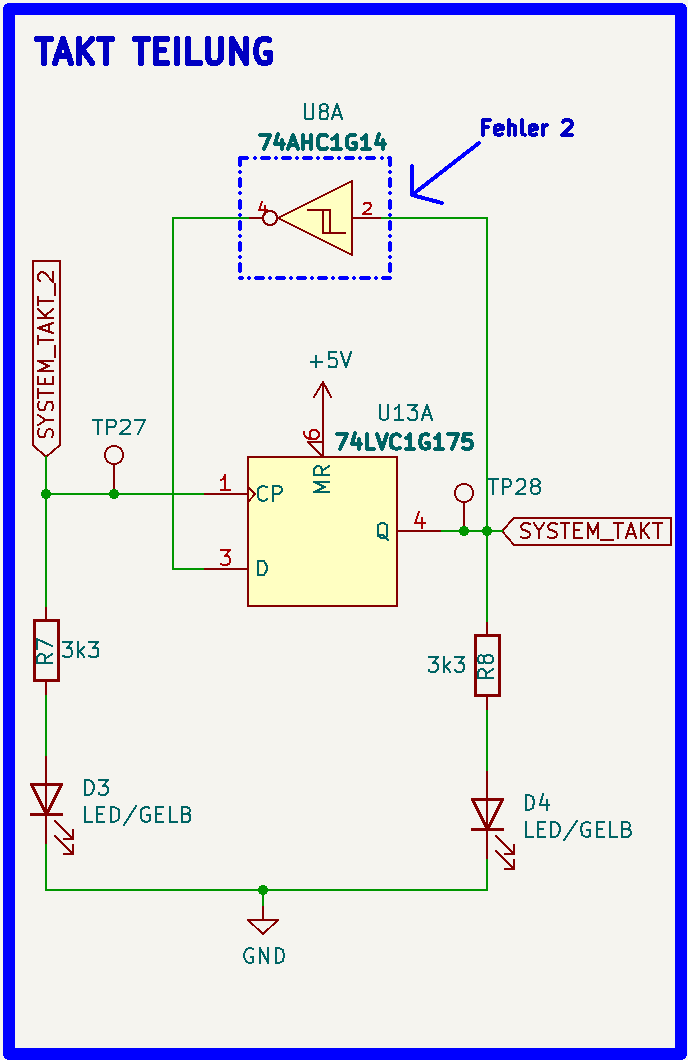
\includegraphics[width=7cm]{Bilder/Taktteilung.png}
\end{center}

Für einen folgenden Schaltungsteil wird ein Takt, welcher die doppelte Frequenz des Messtaktes besitzt benötigt. Dazu wird der Grundtakt durch zwei geteilt und als Messtakt verwendet. Der externe oder interne Grundtakt wird vom folgenden Schaltungsteil verwendet.
\\
D3 und D4 geben ein optisches Feedback des Mess- und Grundtaktes. 


\subsection{Dezimal Zähler}

\subsubsection{Messung Starten}

\begin{center}
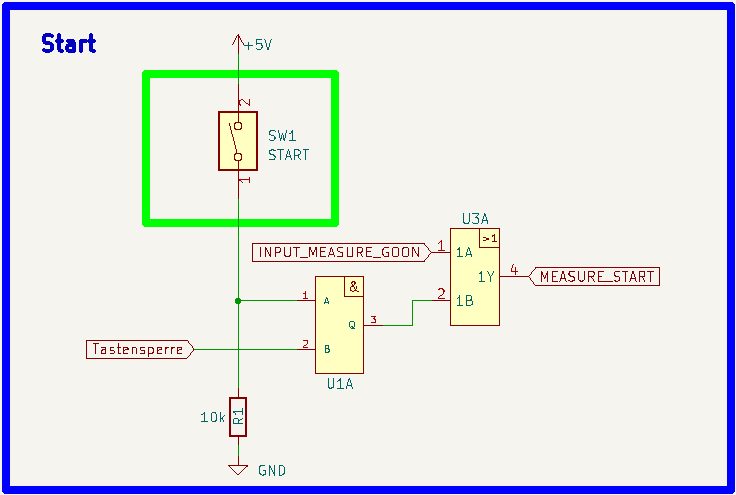
\includegraphics[width=12cm]{Bilder/Start.png}
\end{center}

Die Messung kann über Betätigung des Tasters SW1 (START) oder über ein externes Signal (Label: INPUT MEASURE GOON) gestartet werden. Befindet sich die Messplatine im \glqq Master Mode \grqq{} (\textbf{Master Mode:}  Grundtakt = Interner Takt \textbf{Slave Mode:} Grundtakt = Externer Takt), so kann die Messung durch den Tasters SW1 gestartet werden. Befindet sich die Messplatine im \glqq Slave Mode \grqq{} so kann nur durch ein externes Signal die Messung gestartet werden. Der Taster SW1 (START) ist gesperrt.


\subsubsection{Reset}

\begin{center}
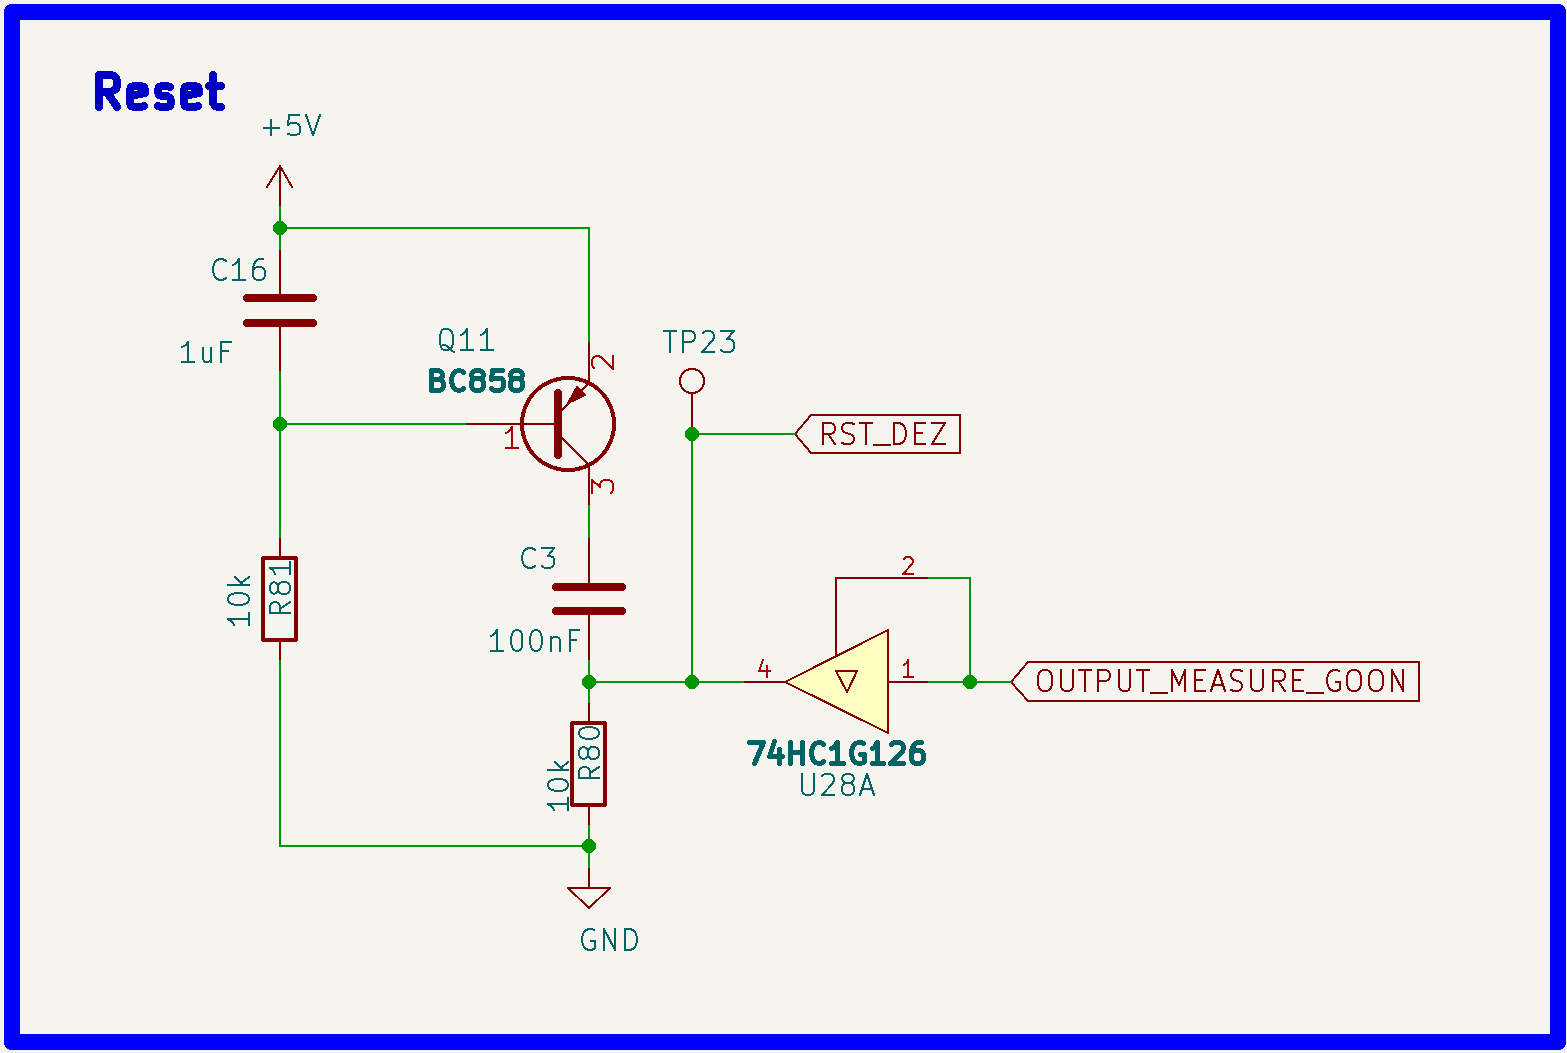
\includegraphics[width=12cm]{Bilder/Reset.png}
\end{center}

Die Aufgabe der folgenden Schaltung besteht darin, kurze Zeit nach dem Einschalten einen Reset-Impuls für ausgewählte Schaltungsteile zu generieren. Wird dies nicht gemacht, so kann es unter zufälligen Umständen sein, dass die Messung nicht gestartet werden kann.
\\
\\
Im Einschaltmoment fließt Strom über C16 und R81. C16 liegt dabei parallel zu den Anschlüssen \glqq Emitter und Basis\grqq{} des PNP-Transistors Q11. Da im Einschaltmoment C16 als Kurzschluss zu betrachten ist, liegen Emitter und Basis auf dem selben Potential. Ein Stromfluss ist daher nicht möglich und der Transistor Q11 sperrt. C16 beginnt sich über die Zeit langsam aufzuladen. Liegt ein bestimmtes Spannungspotetial über C16 an (ca. 0,7V $U_{BE}$), so ist ein Stromfluss durch die Basis möglich. Nach einer bestimmten Verzögerung ist nun auch ein Stromfluss durch den Transistor Q11, durch den Kondensator C5 und dem Widerstand R80) möglich. Da C3 ebenfalls im ersten Moment als Kurzschluss zu betrachten ist, fällt über R80 angfänglich ein 5V pegel ab. Die Spannung über C3 baut sich dabei sehr schnell auf, was einen kurzen Nadelimpuls zur folge hat. Das globale Label \glqq RST DEZ\grqq{} resetet die Schaltungsteile.  
\\
\\
Das IC U28A (Tri-State IC) dient zur Stromkreisentkopplung und soll beim Resetvorgang einen Kurzschluss vermeiden. Der Strom kann nur in eine Richtung fließen.

\newpage
\subsubsection{Controlling}

\begin{center}
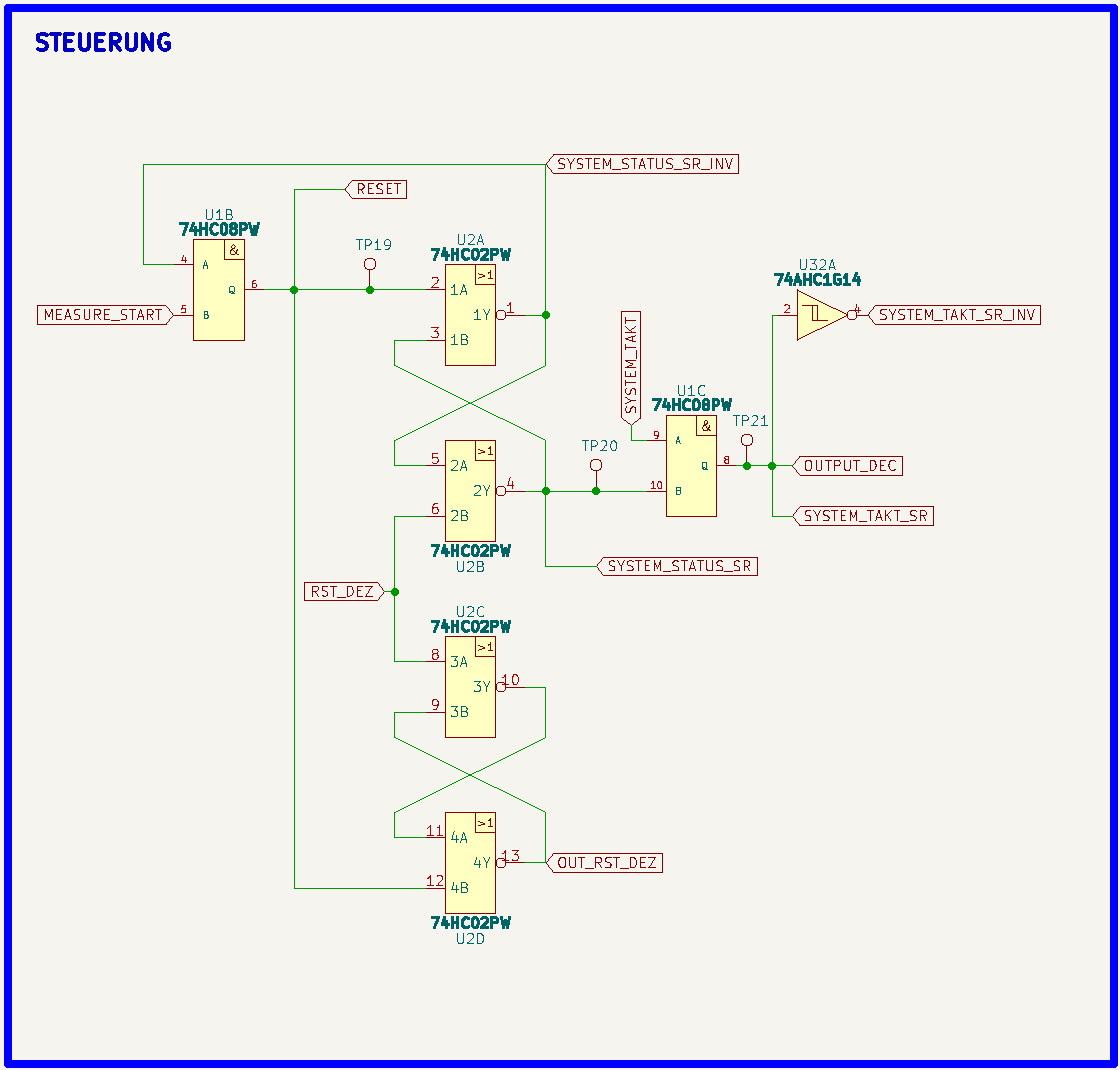
\includegraphics[width=12cm]{Bilder/Controlling.png}
\end{center}

Durch die voran gegangene Schaltung, welche die FlipFlops \textbf{FF1:} U2A und U2B \textbf{FF2:} U2C und U2D in die definierten Ausgangszustände bringt, kann nun ein einwandfreier Start der Messung durchgeführt werden. 
\\
\\
Zum Start der Messung hat das IC U2A einen Ausgangsseitigen High-Pegel vorzuweisen. Der Ausgang ist dabei auf den Steuereingang des TOR-Gatter zurückgeführt.
\\
Das TOR-Gatter U1C erfährt an seinem Steuereingang Pin 10 einen Low-Pegel. Der anliegende Messtakt wird gesperrt.
\\
An dem Ausgang des IC U2D liegt ein Low-Signal an. Dieses Low-Signal resetet die folgende Schaltung dauerhaft.  
\\
\\
Ein High-Signal am Pin 5 (U1B \textbf{LABEL:} MEASURE START) wird auf den Ausgang übertragen. Das an TP19 zu messende High-Signal bleibt so lange aktiv, wie das folgende FlipFlop (U2A und U2B) für das Rücksetzen des Ausganges Pin 1 bzw. für das Setzen des Ausganges Pin 4 benötigt (Gatterlaufzeit). Ein eventuell prellendes Signal an U1B wird somit sofort unterdrückt.
\\
Das High-Signal an TP20 führt dazu, dass der Messtakt an Pin 8 (U1C) auf den Ausgang übertragen wird. 
\\ 
Der Nadelimpuls an TP19, führt somit zu einem Rücksetzen des IC U2D. Das daraus resultierende Low-Signal gibt die Folgeschaltung somit frei.

\newpage
\subsubsection{Dezimalzähler}

\begin{center}
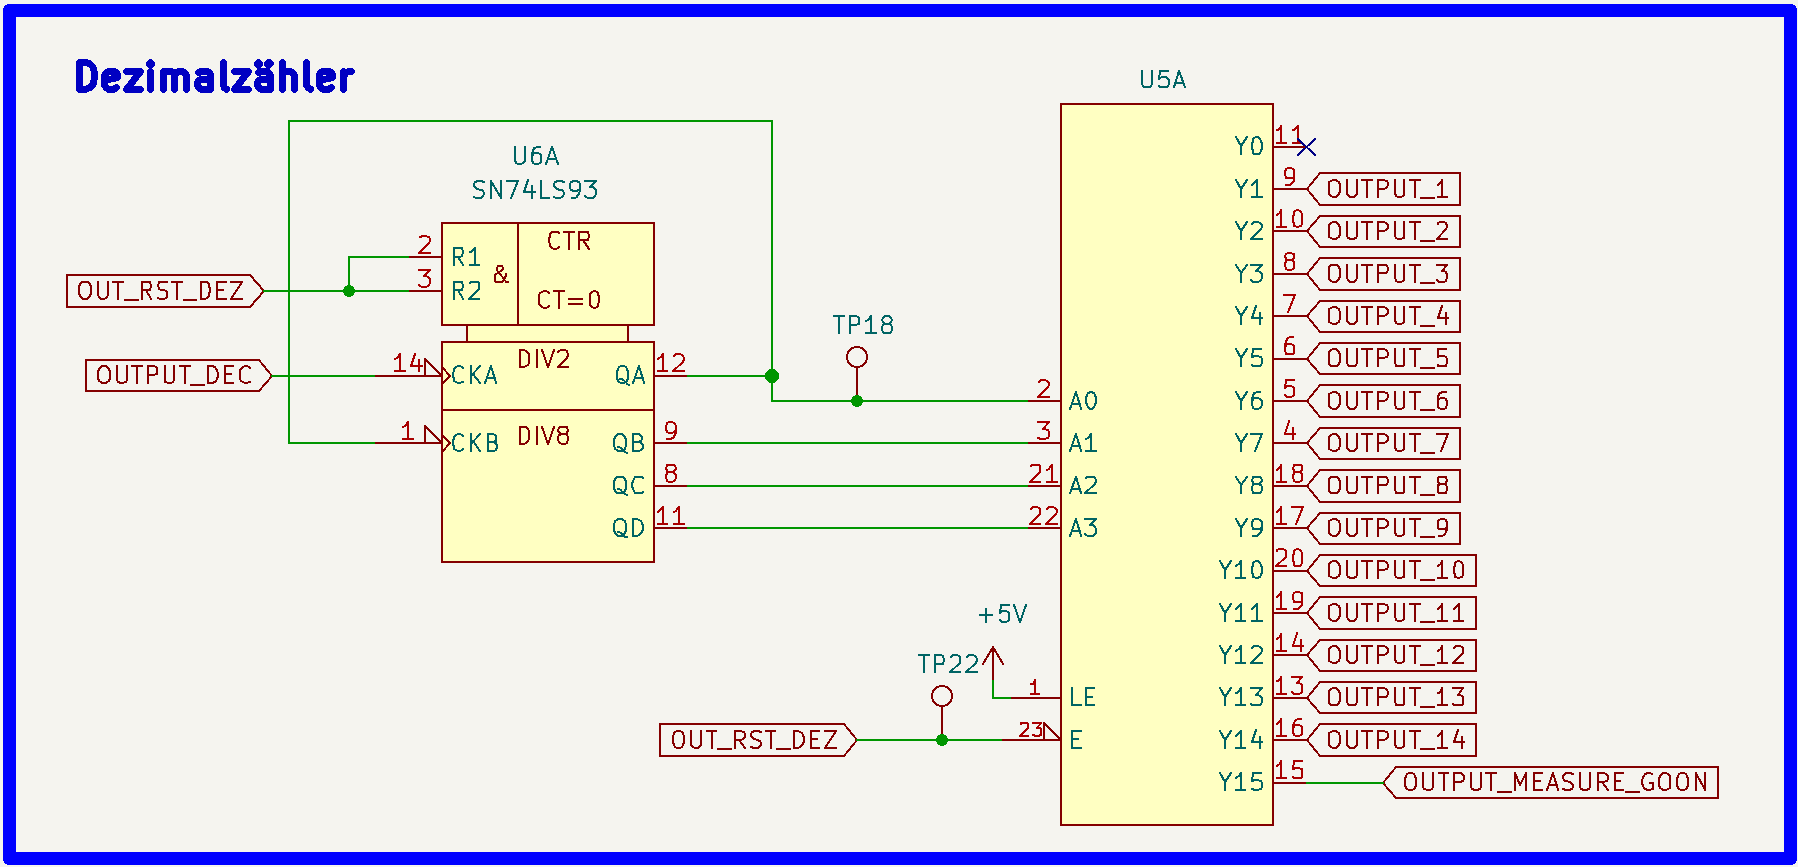
\includegraphics[width=16cm]{Bilder/Dezimalzähler.png}
\end{center}

\newpage
\subsection{Leitungstreiber und Umschaltung}

\begin{center}
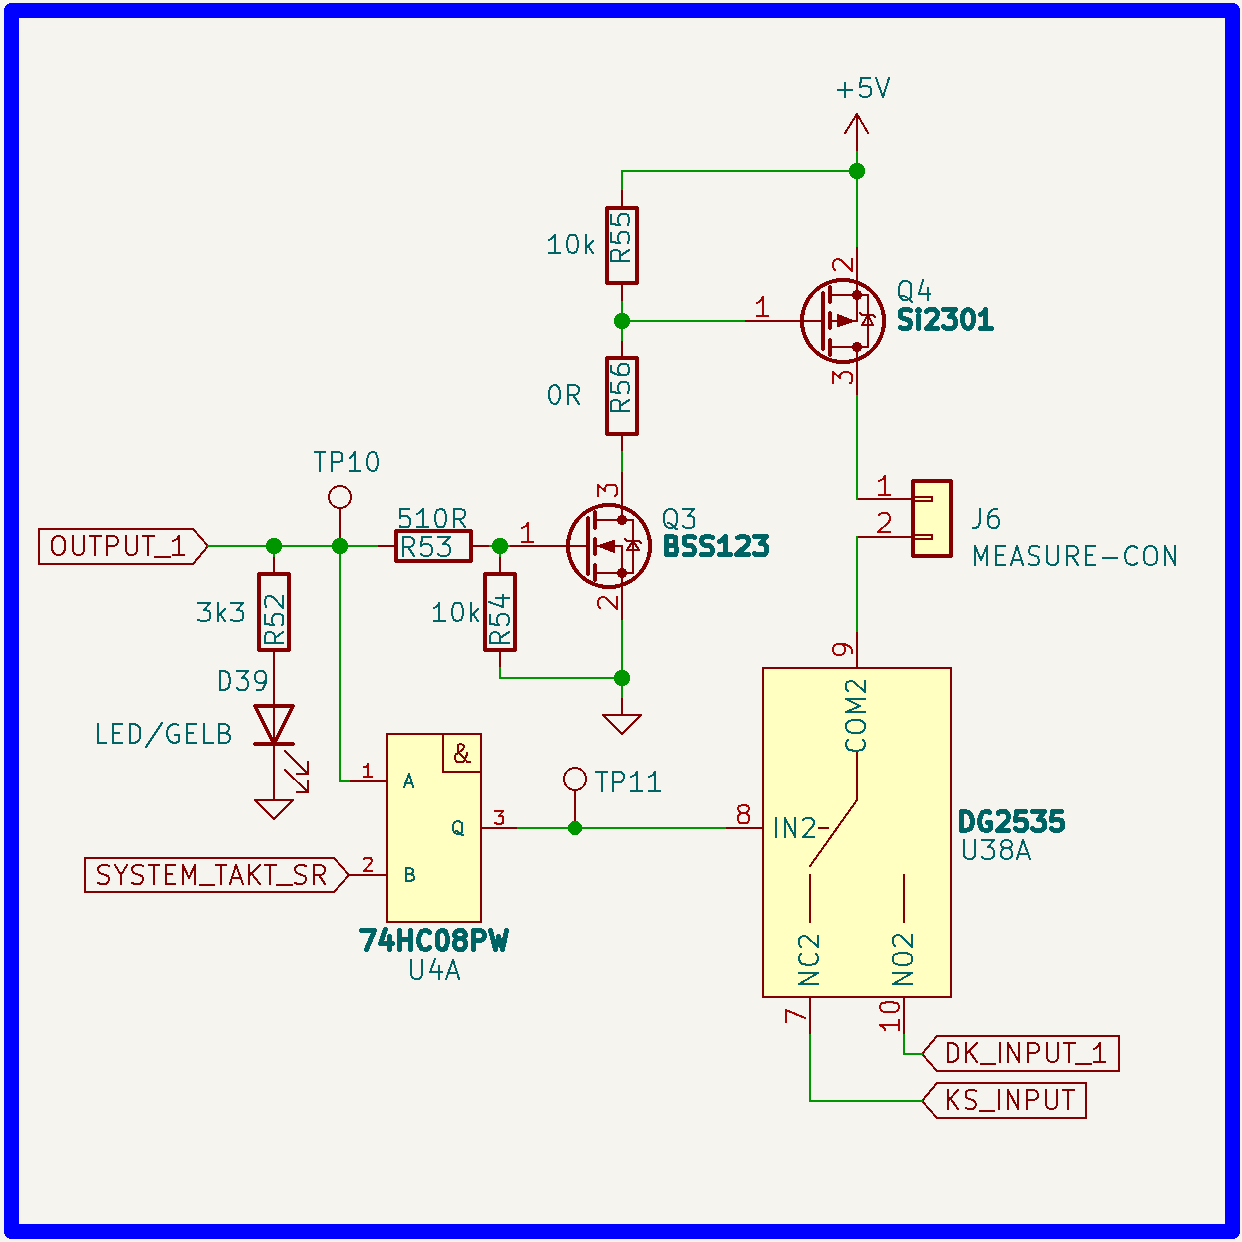
\includegraphics[width=12cm]{Bilder/Leitungstreiber.png}
\end{center}

\newpage
\subsection{Durchgangs und Kurzschlussprüfung}

\begin{center}
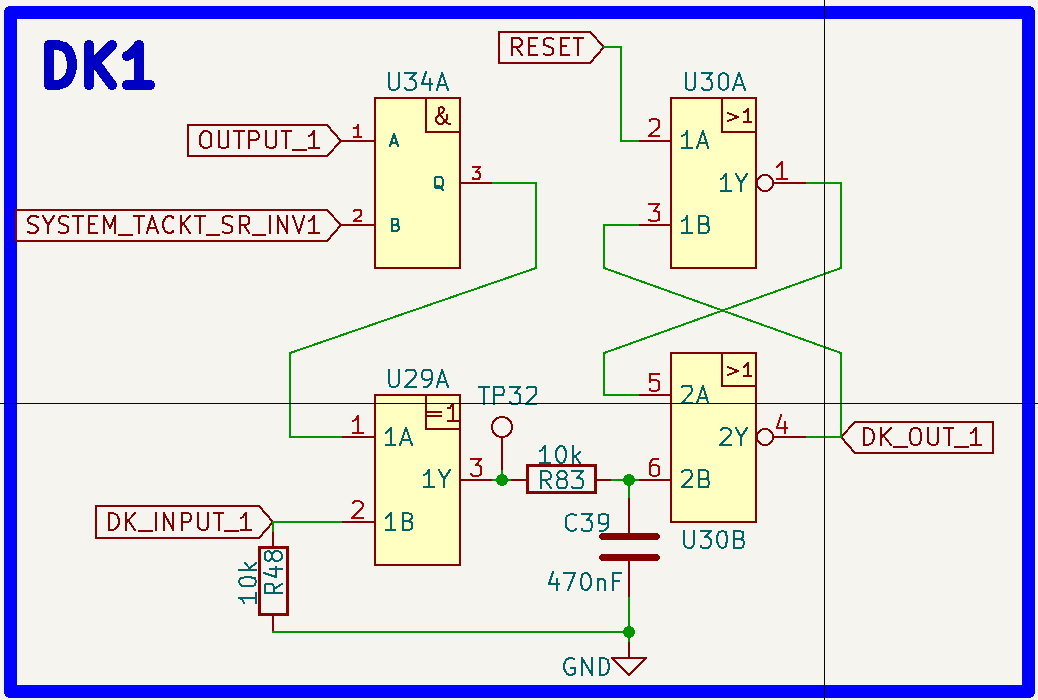
\includegraphics[width=12cm]{Bilder/Durchgangsprüfung.png}
\end{center}

\newpage
\subsection{Konstantstrommessung}

\subsubsection{Konstantstrommessung}
\begin{center}
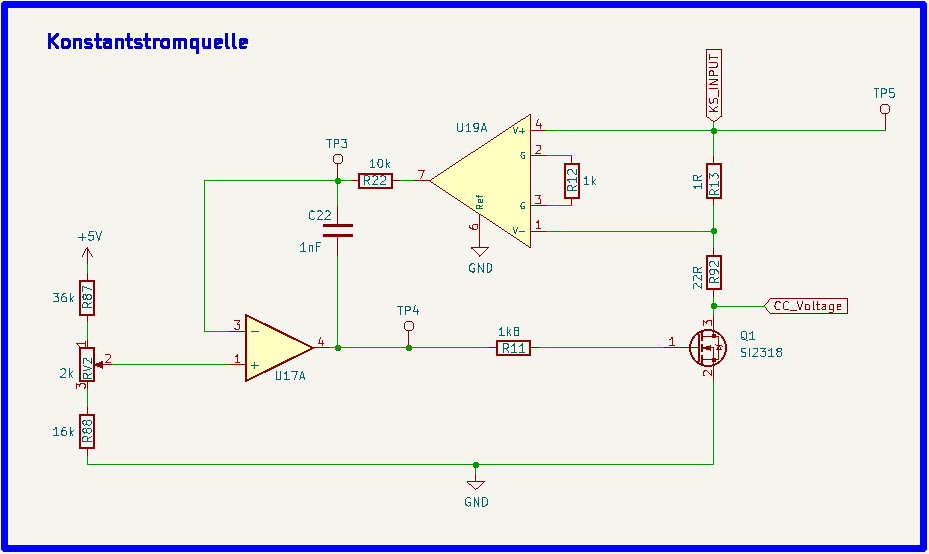
\includegraphics[width=12cm]{Bilder/Konstantstromquelle.png}
\end{center}

\newpage
\subsubsection{Auswertung}
\begin{center}
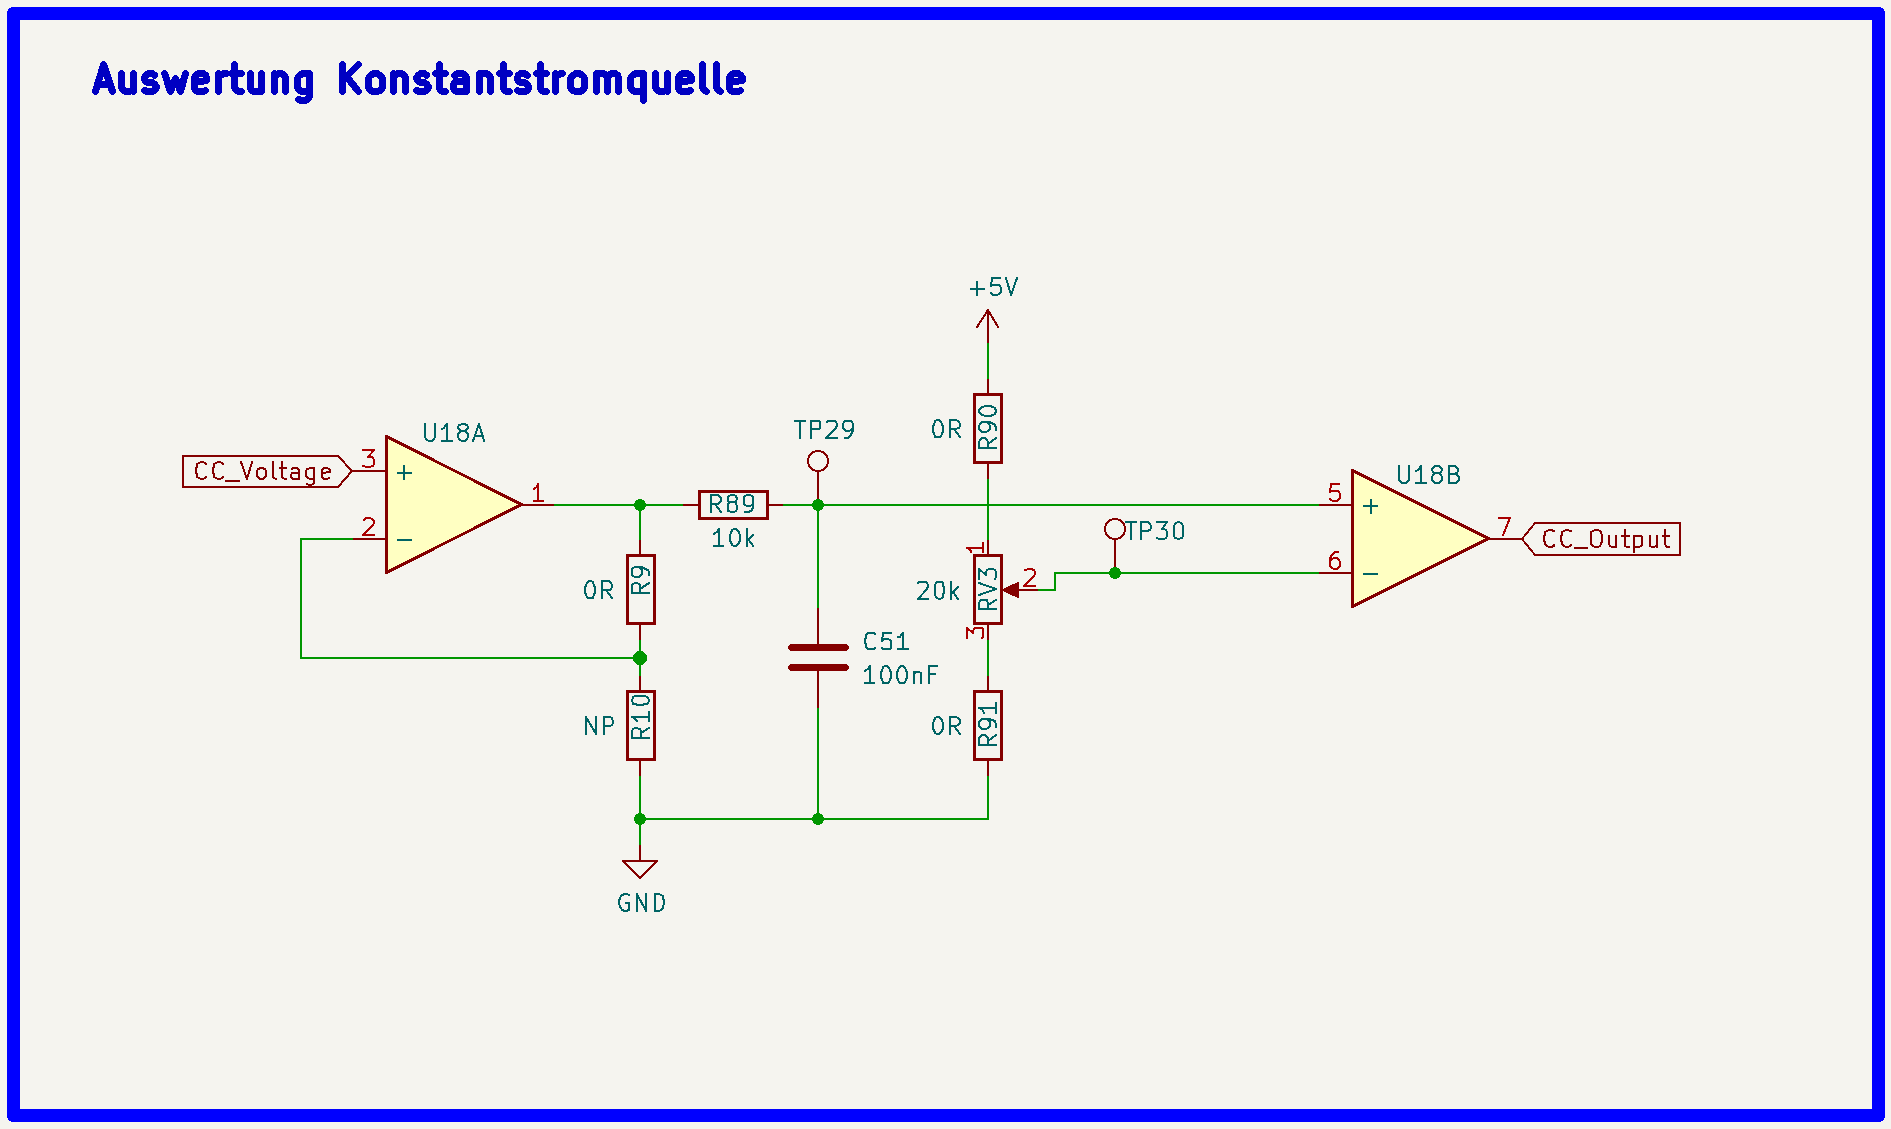
\includegraphics[width=15cm]{Bilder/Auswertung.png}
\end{center}

\newpage
\subsubsection{Ausgabe}
\begin{center}
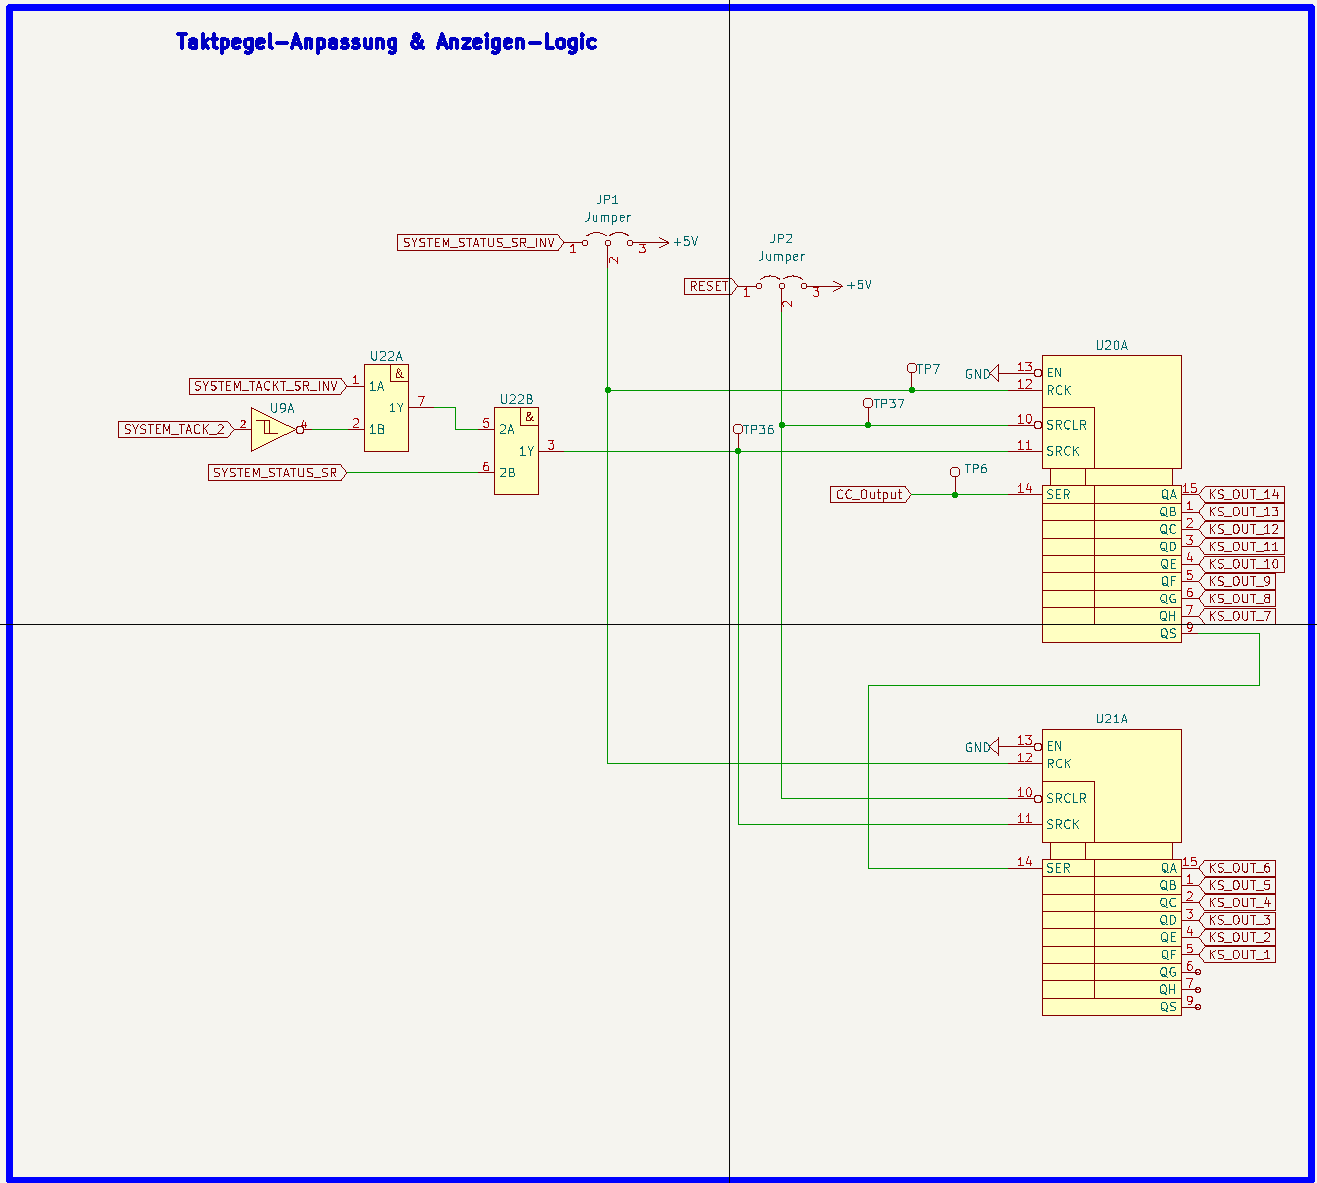
\includegraphics[width=15cm]{Bilder/Anzeige-Logik.png}
\end{center}

\newpage
\subsection{Anzeige}


\begin{center}
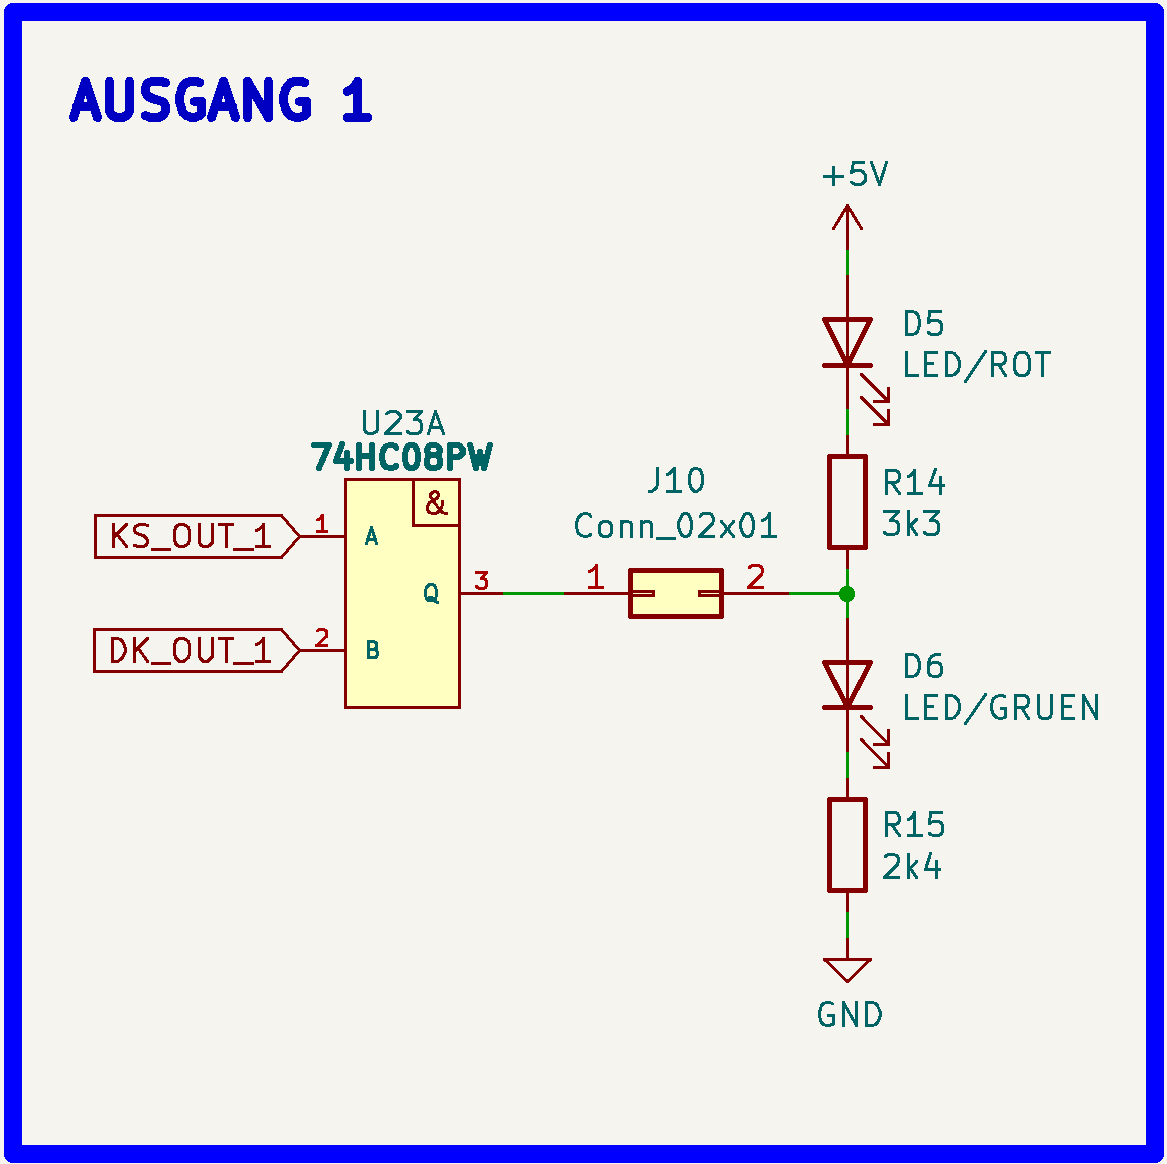
\includegraphics[width=12cm]{Bilder/Anzeige.png}
\end{center}




\end{document}